\shorthandoff{"}
\chapter{Methodik}
\label{ch:methodik}

\section{Art der Forschung}
\label{ch:methodik:art}
Die vorliegende Master-Thesis verfolgt das Ziel, die folgende Forschungsfrage zu beantworten: xyz.

Um diese Fragestellung in Form eines A/B-Tests zu untersuchen, wird eine quantitative Forschungsarbeit in Form eines Experiments durchgeführt. Hierfür werden zwei Versionen eines Empfehlungssystems zur Besetzung offener Projektpositionen entwickelt. Eine der beiden Anwendungen soll einen unilateralen, die andere einen bilateralen Ansatz verfolgen. Beide Empfehlungssysteme erhalten als Eingabe dieselben offenen Projektpositionen. Für diese Stellen sortieren die Anwendungen die vorhandenen Mitarbeiter des Betriebs und geben diese in Form einer Liste zurück. Die Ausgaben beider Systeme werden Projektmanagern des Unternehmens vorgelegt. Daraufhin bewerten diese auf einer vordefinierten Skala, welche Arbeitsleistung sie von denen in der vorliegenden Reihenfolge dargestellten Mitarbeitern erwarten. Die Angestellten erhalten die Beschreibungen der offenen Projektpositionen und bewerten ebenfalls auf einer vordefinierten Skala, wie zufrieden sie voraussichtlich mit der Tätigkeit auf den vorliegenden Projektpositionen sein werden. Hierbei wird überprüft, ob eine hohe erwartete Zufriedenheit des Angestellten mit einer hohen Positionierung in den Ergebnislisten der Empfehlungssysteme korreliert.

\section{Versuchsaufbau}
\label{ch:methodik:versuchsaufbau}
Durchgeführt wird das Experiment mit Projektmanagern und Mitarbeitern der EXXETA AG mit Hauptsitz in Karlsruhe. Das Unternehmen ist spezialisiert auf IT-Beratungsleistungen und arbeitet vorrangig projektbasiert. Passende Angestellte zu offenen Projektpositionen zuzuordnen ist in diesem Betrieb dementsprechend eine häufig auftretende Aufgabe. Daher liegen Informationen über die Mitarbeiter bereits in einer strukturieren Form vor. Diese Daten dienen im Experiment als Eingabe für einen unilateralen Empfehlungsalgorithmus.

\subsection{Unilaterales Empfehlungssystem}
\label{ch:methodik:versuchsaufbau:unilateral}
Die Mitarbeiter der EXXETA AG pflegen ihre Kompetenzen in einem Intranet. Dort steht eine Liste mit 551 Fähigkeiten wie beispielsweise "Java", "DSGVO" und "Digitale Transformation" zur Verfügung. Diese können die Angestellten über die in Abbildung \ref{fig:methodik:versuchsaufbau:daten:abb1} dargestellte Skala bewerten.

\begin{figure}[h]
	\centering
	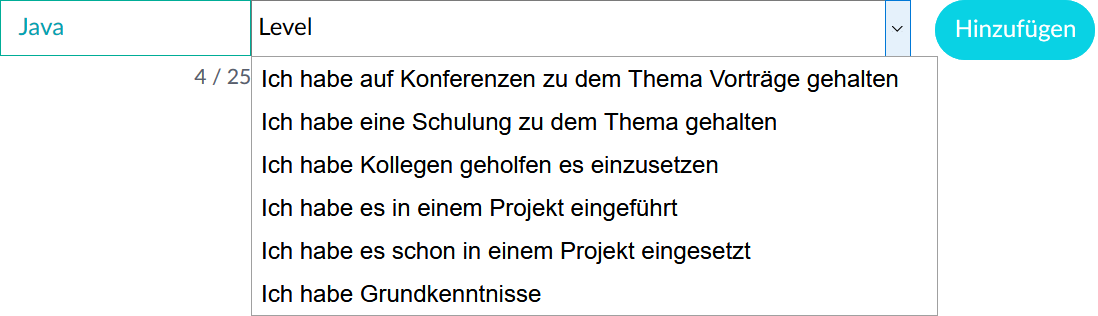
\includegraphics[width=1\textwidth]{gfx/skill-level.png}
	\caption{Hinzufügen einer Fähigkeit mit Angabe des entsprechenden Kenntnisniveaus im EXXETA-Intranet}
	\label{fig:methodik:versuchsaufbau:daten:abb1}
\end{figure}

Die in Abbildung \ref{fig:methodik:versuchsaufbau:daten:abb1} dargestellten Abstufungen werden beim Speichern in ganzzahlige Werte von null ("Ich habe Grundkenntnisse") bis sechs ("Ich habe auf Konferenzen zu dem Thema Vorträge gehalten") übertragen.

Um im unilateralen Empfehlungssystem Mitarbeiter für offene Projektpositionen vorzuschlagen, wird die Katz-Zentralität angewendet. Dieser speicherbasierte Graphenalgorithmus wurde in Kapitel \ref{ch:empfehlungssysteme:cf:speicherbasiert} vorgestellt. Ein Nutzen dieses Ansatzes ist die zuverlässige Lösung des Sparsity Problems. Vorteilhaft gegenüber modellbasierten Methoden ist außerdem die Langlebigkeit des Verfahrens. Sollten sich nach Durchführung des Experiments Daten im Unternehmen signifikant verändern oder neue Kompetenzen im Intranet hinzugefügt werden, ist der speicherbasierte Ansatz weiterhin unverändert anwendbar. Die dabei zu erwartende hohe Komplexität ist in der vorliegenden Problemstellung tolerierbar, da sich zum Zeitpunkt des Experiments unter 1.000 Mitarbeiter im Unternehmen befinden.

Um neben dem Sparsity Problem auch den Kaltstart zu beheben, werden zusätzlich zu den Fähigkeiten der Mitarbeiter auch deren Teamzuordnungen in Form eines hybriden Ansatzes beachtet. Bei der EXXETA AG arbeiten stets Mitarbeiter in einem Team, welche ähnliche Kompetenzen beherrschen. Der Leiter des Teams ist eine fachliche Führungskraft, dessen Fähigkeiten in der Regel repräsentativ für sein Team sind. Seine Kompetenzen sind jedoch stärker ausgeprägt. Um Rechenleistung einzusparen, werden die Teams nicht als zusätzliche Knoten in den Graphen eingefügt. Die Beziehungen werden stattdessen über direkte Kanten zwischen Kollegen dargestellt. Das Kantengewicht von Teammitglieder zu Teammitglied beträgt eins und das Gewicht von Teammitglied zu seinem Manager zwei. Über diesen Ansatz sind alle Teammitglieder schwach miteinander verbunden, sodass auch für Mitarbeiter ohne vergebene Bewertungen aussagekräftige Beurteilungen bestimmt werden können. Außerdem erhalten die Teammanager durch das höhere Kantengewicht eine stärkere Zentralität im Graphen.  Daher profitieren sämtliche Teammitglieder transitiv von den hinterlegten Fähigkeiten ihres Managers.

Die Fähigkeitsbewertungen und Teamzuordnungen können für alle Mitarbeiter der EXXETA AG über eine \acsu{REST}-Schnittstelle in Form von \acsu{JSON} aus dem Intranet abgefragt werden. Quellcode \ref{qc:methodik:versuchsaufbau:daten:qc1} zeigt beispielhaft einen Auszug aus den zurückgegebenen Daten von John Doe aus Tabelle \ref{tbl:empfehlungssysteme:arbeitsweise:tbl1}.

In Quellcode \ref{qc:methodik:versuchsaufbau:daten:qc1} ist zu erkennen, dass eine Bewertung von eins in Tabelle \ref{tbl:empfehlungssysteme:arbeitsweise:tbl1} einer Beurteilung von null im zurückgegebenen \ac{JSON} entspricht. Damit ein Kantengewicht von null ausschließlich nicht vergebene Kompetenz-Einschätzungen symbolisiert, werden die Bewertungen vor Berechnung der Katz-Zentralität um eins erhöht.

Die Darstellung der Kompetenzen und Teamzuordnungen der Mitarbeiter aus Tabelle \ref{tbl:empfehlungssysteme:arbeitsweise:tbl1} in der Form eines bipartiten Graphen ist in Abbildung \ref{fig:methodik:versuchsaufbau:unilateral:abb1} zu erkennen. In der Grafik wird Jane Doe als Teammanager betrachtet.

\begin{figure}[h]
	\centering	
	\begin{tikzpicture}[node distance={32mm}, thick, main/.style = {draw, circle}] 
		\node[main, fill=itemcolor] (MongoDB) {$MongoDB$}; 
		\node[main, fill=itemcolor] (Python) [below right of=MongoDB] {$Python$}; 
		\node[main, fill=itemcolor] (MySQL) [above right of=Python] {$MySQL$}; 
		\node[main, fill=itemcolor] (Java) [below right of=MySQL] {$Java$}; 
		\node[main, fill=itemcolor] (HDFS) [above right of=Java] {$HDFS$}; 
		\node[main, fill=itemcolor] (Spark) [below right of=HDFS] {$Spark$};
		
		\node[main, fill=usercolor] (Jane) [above right of=MongoDB] {$Jane D.$}; 
		\node[main, fill=usercolor] (John) [above left of=HDFS] {$John D.$}; 
		\node[main, fill=usercolor] (Max) [below of=MySQL] {$Max M.$};
		\node[main, fill=usercolor] (Erika) [above right of=HDFS] {$Erika M.$}; 
		
		\draw (Jane) -- node[midway, right] {4} (Python);
		\draw (Jane) -- node[midway, above] {3} (MySQL);
		\draw (Jane) -- node[midway, above] {3} (MongoDB);
		
		\draw (John) -- node[midway, right] {1} (HDFS);		
		\draw (John) -- node[midway, right] {3} (Java);
		\draw (John) -- node[midway, above] {2} (MySQL);
		
		\draw (Erika) -- node[midway, above] {5} (HDFS);
		\draw (Erika) -- node[midway, left] {3} (Spark);
		
		\draw (Max) -- node[midway, above] {2} (Java);
		\draw (Max) -- node[midway, above] {3} (Python);
		\draw (Max) -- node[midway, right] {1} (MySQL);
		
		\draw (Jane) -- node[midway, above] {2} (John);
		\draw (Jane) -- node[midway, left] {2} (Max);
		\path (Jane) edge[bend left=25] node[midway, above] {2} (Erika);
		
		\draw (John) -- node[midway, right] {1} (Max);
		\draw (John) -- node[midway, above] {1} (Erika);
		
		\path (Max) edge[bend right=40] node[midway, below] {1} (Erika);
	\end{tikzpicture}
	
	\caption{Graph aus Abbildung \ref{fig:empfehlungssysteme:cf:speicherbasiert:abb2} mit zusätzlicher Teamzuordnung}
	\label{fig:methodik:versuchsaufbau:unilateral:abb1}
\end{figure}

\begin{minipage}{\linewidth}
\lstinputlisting[
	language=json,
	caption=Beispiel für ein Mitarbeiter-\acsu{JSON} der \acsu{REST}-Schnittstelle des Intranets der EXXETA AG (Auszug),
	captionpos=b,
	label=qc:methodik:versuchsaufbau:daten:qc1
]{gfx/john.json}
\end{minipage}

Bei der Berechnung der Katz-Zentralität wird auf eine Mittelwert-Zentrierung verzichtet. Aufgrund der klaren Beschreibungen der einzelnen Stufen in Abbildung \ref{fig:methodik:versuchsaufbau:daten:abb1} kann Bias bei der Selbsteinschätzung weitgehend ausgeschlossen werden. Außerdem ist es in der vorliegenden Problemstellung gut möglich, dass einzelne Mitarbeiter ihre Kompetenzen grundsätzlich besser oder schlechter einschätzen als andere Kollegen. Dieser Sachverhalt kann insbesondere auf längere Berufserfahrung zurückgeführt werden.

\newpage
Sucht ein Projektmanager nach passenden Mitarbeitern für eine offene Projektposition, definiert dieser zunächst die für die Position benötigten Fähigkeiten mit

Zu erhebende Daten:\\
- Für jeden Mitarbeiter erheben: Wichtigkeit (true/false) --> Auch für Dinge, die man noch nicht kann\\
- Für jeden Mitarbeiter erheben: Welche Auswirkung hat es, wenn im Projekt nicht ausgelastet (Kurve A bis C) --> Alle drei Antwortmöglichkeiten positiv formulieren --> z.B. Freiräume nutzen

Erstellen des Graphen:\\
- Aus Skills (kollaboratives Filtern) und Teamzuordnung (Inhaltsbasiertes Filtern) einen tripartiten Graphen erstellen\\

Eingabe der offenen Projektposition:\\
- Benötigt: Fähigkeiten und Wichtigkeit (Boolean)

Algorithmus:\\
- Berechnung der Katz-Zentralität\\
- Für jeden relevanten Mitarbeiter auf Basis von Abbildung \ref{fig:methodik:abb2} den finalen Wert bestimmen --> Hierbei je nach Wichtigkeit die Kurve stauchen --> Wenn für Projektmanger wichtig, die durchgezogene Linie doppelt so steil; Wenn für Mitarbeiter wichtig, rechte Seite doppelt so steil; Auswahl der Kurve anhand der Information des Mitarbeiters\\
- Summe für alle Fähigkeiten eines Projektes für jeden Mitarbeiter berechnen

\begin{figure}[h]
	\centering
	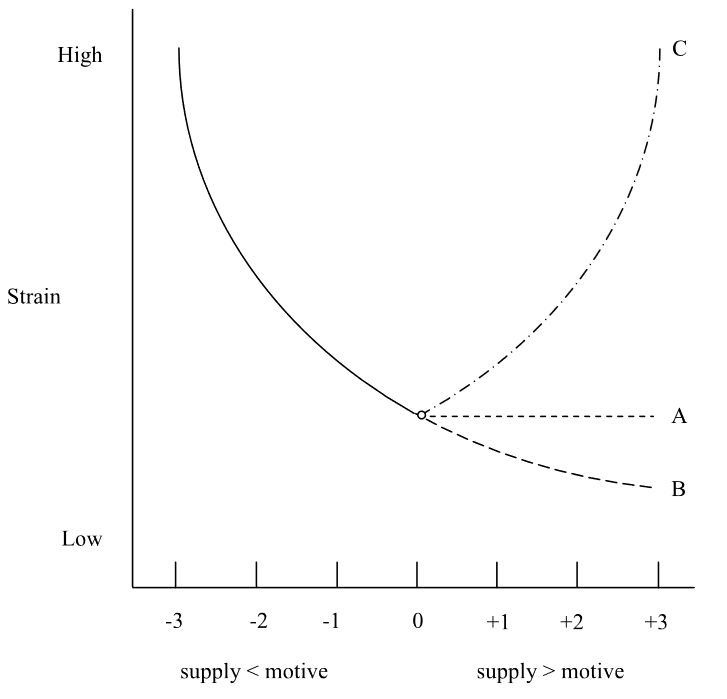
\includegraphics[width=0.75\textwidth]{gfx/ueberschuss_supply_motive.png}
	\caption{Auswirkungen eines Bedürfnisse-Angebote Misfits \cite[S. 23]{edwards:2008}\\(Bearbeitet von \myName)}
	\label{fig:methodik:abb2}
\end{figure}

- Algorithmus einmal durchführen mit Wichtigkeiten und einmal ohne (bilateral vs. unilateral)\\
- Ausgabe der sortierten Liste (mit allen Mitarbeitern (zB 25))\\
- Eingabe der Projektposition und Algorithmus für jede Projektposition wiederholen

\section{Geplante Evaluation}
\label{ch:methodik:evaluation}
Evaluation für Projektmanager:\\
- Erhält für jedes Projekt beide Listen und gibt auf einer Skala von 1 bis 5 an, wie hoch der die Leistung der empfohlenen Mitarbeiter in diesem Projekt einschätzen würde

Evaluation für Mitarbeiter:\\
- Jeder Mitarbeiter muss für jedes Projekt auf einer Skala von 1 bis 5 bewerten, wie zufrieden er wäre, wenn er darin arbeiten würde\\
- Ergebnisliste wird in Intervalle geteilt --> z.B. Zufriedenheit 5 bedeutet bei 25 Teilnehmern, dass der Nutzer im ersten Intervall sein muss --> Abweichung bestimmen --> Je weniger Abweichung, desto besser --> Durchschnittliche Abweichung von unilateral und bilateral vergleichen

Frage:\\
- Sollte Manager überhaupt Wichtigkeiten angeben?\\
	- Fähigkeiten sind Angebote und Wichtigkeiten Nachfrage\\
- Ist das Vergleichs-Vorgehen unilateral?\\
- Welche Daten müssen in den Anhang der Thesis?
\shorthandon{"}
